\chapter{Results}
<reproducer resultater fra Arayns thesis>
Egne forsøg med SPN og mixture regression


\subsection{regression benchmark}
We will benchmark our different regression models againt a simple emperical mean and
emperical std. normal distribution benchmark, 
$$p(y|x\mathcal{D}) = \mathcal{N}(y| \bar{\textbf{y}} , \bar{\sigma}^2 (\textbf{y}))$$

where $\bar{\textbf{y}} = \frac{1}{n}\sum_{i=1}^n \textbf{y}_i $ and 
$\bar{\sigma}^2 (\textbf{y})) = \frac{1}{n-1}\sum_{i=1}^n (\textbf{y}_i-\bar{\textbf{y}})^2 $
this is however not a good model for Bayesian optimization, as it will not provide a
new candidate point, as all points are equally good. 


\section{Mixture regression on simple functions}
Choosing a good set of design parameters is crucial, 
the manipulation... 

\begin{figure}[h]
    \caption{Regression plot for one problem with all dims: Number of data points / dims, mean squared error, with bayesline mean prediction}
\end{figure}

\begin{figure}[h]
    \caption{Regression plot for anther problem}
\end{figure}

% \begin{figure}[h]
%     \centering
%         \begin{tabular}{c|ll|l|l}
%         \multicolumn{1}{l|}{Problem 2D} & Winner (rel error)                                              & Second                                                                                  & Third                              &  \\ \cline{1-4}
%         f1                                                      & \multicolumn{1}{c|}{GP (0.2)}                                                           & \multicolumn{1}{c|}{\begin{tabular}[c]{@{}c@{}}Neural Network\\ (0.00001)\end{tabular}} & \multicolumn{1}{c|}{Naive (0.002)} &  \\
%         f2                                                      & \multicolumn{1}{c|}{Naive (0.002)}                                                      &                                                                                         &                                    &  \\
%         f3                                                      & \multicolumn{1}{c|}{\begin{tabular}[c]{@{}c@{}}Neural Network\\ (0.00001)\end{tabular}} &                                                                                         &                                    &  \\
%         f4                                                      & \multicolumn{1}{l|}{}                                                                   &                                                                                         &                                    &  \\
%                                                                 & \multicolumn{1}{l|}{}                                                                   &                                                                                         &                                    & 
%         \end{tabular}
%     \caption{Table summarizing for all problems}
% \end{figure}

\begin{figure}[h]
    \centering
    \begin{tabular}{llllll}
\hline
          & f1         & f2             & f3          & f4          & f5         \\
\hline
 BO\_numpy & 4.62(13.0) & 897.13(39.0)   & 2.07(36.0)  & 10.14(39.0) & 0.03(28.0) \\
 BO\_BOH   & 0.33(32.5) & 552.83(27.0)   & 5.51(33.0)  & 10.33(37.0) & 0.03(28.0) \\
 BO\_Gaus  & 0.89(8.0)  & 21.48(31.5)    & 21.86(21.0) & 16.32(25.5) & 0.03(22.5) \\
 BO\_Naiv  & 3.25(9.0)  & 72571.84(28.0) & 19.41(15.0) & 19.61(8.5)  & 4.35(21.0) \\
 BO\_em    & 1.23(24.5) & 455.28(10.0)   & 6.74(8.5)   & 5.98(30.5)  & 6.00(22.5) \\
\hline
\end{tabular}
    \caption{Distance to optima $f(x^{best})-f^*$ using Bayesian optimization with different surrogates
    and using expected improvement with a budget of $40$ samples for group 1: "5 separable functions"}
\end{figure}

\begin{figure}[h]
    \centering
    \begin{tabular}{lllll}
\hline
          & f6         & f7         & f8          & f9          \\
\hline
 BO\_numpy & 1.31(28.0) & 2.65(10.5) & nan(nan)    & nan(nan)    \\
 BO\_BOH   & 0.05(33.0) & 1.68(17.0) & 10.70(16.0) & 2.31(39.0)  \\
 BO\_Gaus  & 6.53(32.0) & 0.60(12.0) & 1.14(18.8)  & 0.27(25.0)  \\
 BO\_Naiv  & 4.74(20.0) & 4.71(25.5) & 11.87(2.0)  & 20.09(15.5) \\
 BO\_em    & 5.43(20.5) & 1.97(24.5) & 5.11(24.0)  & 68.97(8.0)  \\
\hline
\end{tabular}
    \caption{Distance to optima $f(x^{best})-f^*$ using Bayesian optimization with different surrogates
    and using expected improvement with a budget of $40$ samples for group 2: "4 functions with low or moderate conditioning"}
\end{figure}
\begin{figure}[h]
    \centering
    \begin{tabular}{llllll}
\hline
          & f10            & f11            & f12            & f13         & f14        \\
\hline
 BO\_numpy & nan(nan)       & nan(nan)       & nan(nan)       & nan(nan)    & nan(nan)   \\
 BO\_BOH   & 286.57(30.0)   & 7.48(35.0)     & 2770.49(31.0)  & 4.98(16.0)  & 0.03(30.0) \\
 BO\_Gaus  & 16.52(33.2)    & 638.31(32.0)   & 3033.71(27.8)  & 8.84(23.8)  & 0.01(36.5) \\
 BO\_Naiv  & 49166.58(27.0) & 2848.42(22.0)  & 23714.17(24.0) & 52.21(2.0)  & 0.61(31.0) \\
 BO\_em    & 61391.71(14.0) & 10317.74(20.5) & 673.63(12.5)   & 10.04(19.0) & 0.80(28.0) \\
\hline
\end{tabular}
    \caption{Distance to optima $f(x^{best})-f^*$ using Bayesian optimization with different surrogates
    and using expected improvement with a budget of $40$ samples for group 3: "5 functions with high conditioning, unimodal"}
\end{figure}
\begin{figure}[h]
    \centering
    \begin{tabular}{llllll}
\hline
          & f15         & f16         & f17        & f18         & f19         \\
\hline
 BO\_numpy & nan(nan)    & nan(nan)    & nan(nan)   & nan(nan)    & nan(nan)    \\
 BO\_BOH   & 10.05(20.0) & 9.02(33.0)  & 4.00(4.0)  & 3.55(38.0)  & 2.05(27.0)  \\
 BO\_Gaus  & 17.12(28.0) & 2.86(10.0)  & 3.15(18.5) & 3.26(10.0)  & 13.31(27.0) \\
 BO\_Naiv  & 34.09(20.5) & 3.20(20.5)  & 1.69(9.5)  & 11.72(24.0) & 3.36(5.0)   \\
 BO\_em    & 14.75(24.5) & 10.70(19.0) & 2.27(21.5) & 9.63(13.5)  & 1.99(9.5)   \\
\hline
\end{tabular}
    \caption{Distance to optima $f(x^{best})-f^*$ using Bayesian optimization with different surrogates
    and using expected improvement with a budget of $40$ samples for group 4: "5 multi-modal functions with adequate global structure"}
\end{figure}
\begin{figure}[h]
    \centering
    \begin{tabular}{llllll}
\hline
          & f20        & f21        & f22        & f23        & f24        \\
\hline
 BO\_numpy & nan(nan)   & nan(nan)   & nan(nan)   & nan(nan)   & nan(nan)   \\
 BO\_BOH   & 2.44(34.0) & 1.99(1.0)  & 1.98(25.0) & 2.64(15.0) & 8.98(14.0) \\
 BO\_Gaus  & 1.67(29.0) & 1.23(22.5) & 2.61(12.8) & 5.24(17.2) & 9.99(19.2) \\
 BO\_Naiv  & 2.43(15.5) & 0.27(21.5) & 2.04(4.0)  & 5.15(5.0)  & 7.15(26.5) \\
 BO\_em    & 3.16(17.0) & 1.07(15.0) & 0.90(22.0) & 5.66(13.5) & 3.82(6.5)  \\
\hline
\end{tabular}
    \caption{Distance to optima $f(x^{best})-f^*$ using Bayesian optimization with different surrogates
    and using expected improvement with a budget of $40$ samples for group 5: "5 multi-modal functions with weak global structure"}
\end{figure}

\begin{figure}[h]
    \centering
    \caption{BayesOpt plot: Number of iterations, distance to optima using EI, with bayesline random search}
\end{figure}


\begin{figure}[h]
    \centering
    \begin{minipage}[b]{0.32\textwidth}
     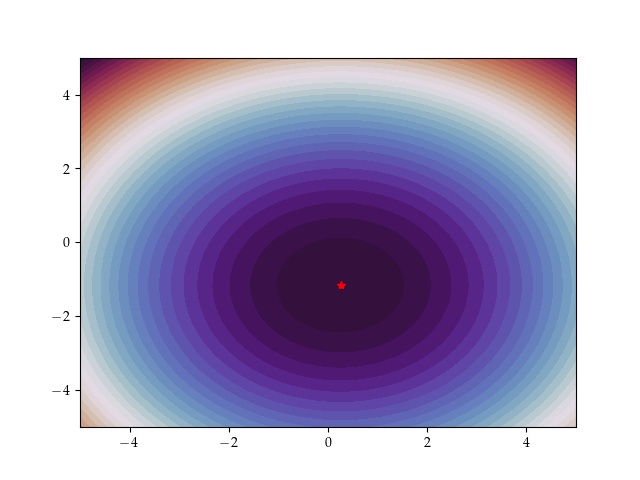
\includegraphics[trim=2.5cm 1.3cm 2.5cm 1.3cm,clip,width=\textwidth]{Figures/coco/f1.png}
    \end{minipage}
    \hfill
    \begin{minipage}[b]{0.32\textwidth}
     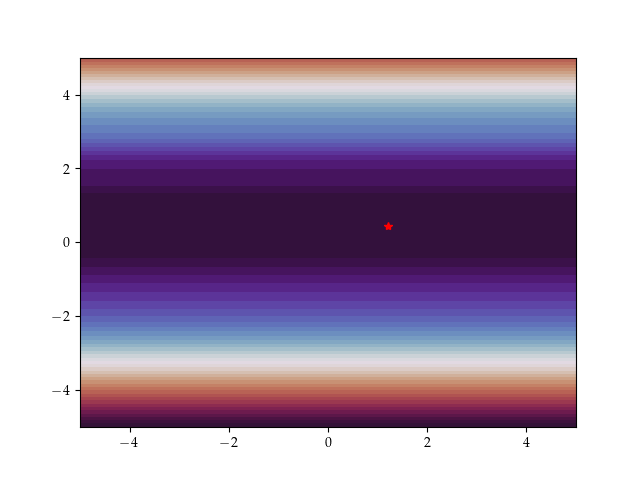
\includegraphics[trim=2.5cm 1.3cm 2.5cm 1.3cm,clip,width=\textwidth]{Figures/coco/f2.png}
    \end{minipage}
    \hfill
    \begin{minipage}[b]{0.32\textwidth}
      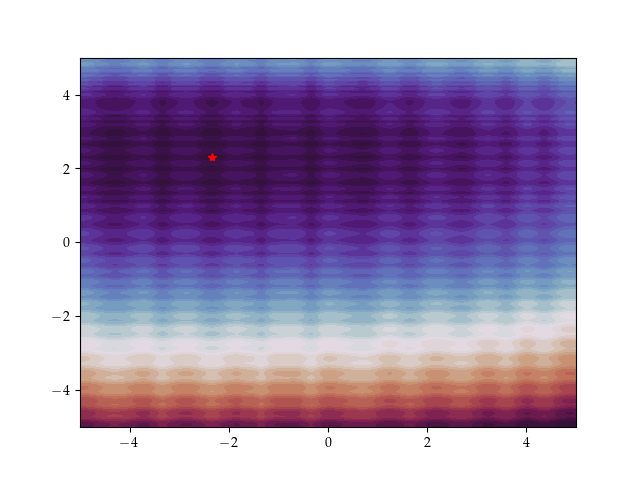
\includegraphics[trim=2.5cm 1.3cm 2.5cm 1.3cm,clip,width=\textwidth]{Figures/coco/f3.png}
      %\caption{Rank}
    \end{minipage}
    
    \begin{minipage}[b]{0.32\textwidth}
      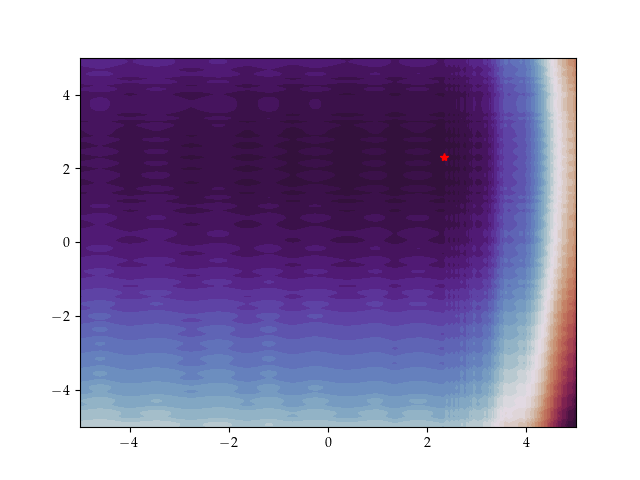
\includegraphics[trim=2.5cm 1.3cm 2.5cm 1.3cm,clip,width=\textwidth]{Figures/coco/f4.png}
    \end{minipage}
    \hfill
    \begin{minipage}[b]{0.32\textwidth}
      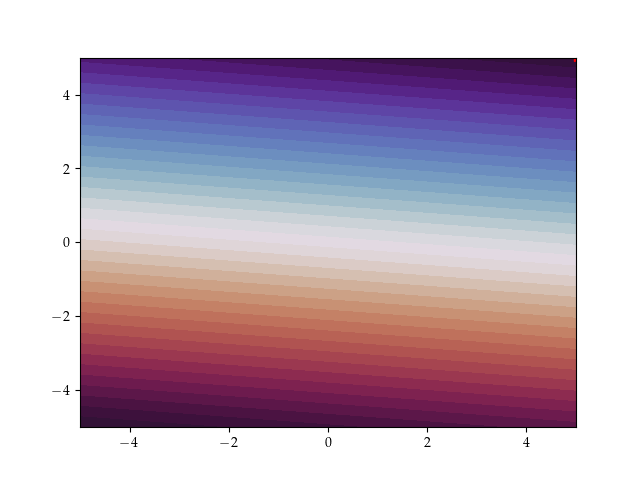
\includegraphics[trim=2.5cm 1.3cm 2.5cm 1.3cm,clip,width=\textwidth]{Figures/coco/f5.png}
    \end{minipage}
    \hfill
    \begin{minipage}[b]{0.32\textwidth}
      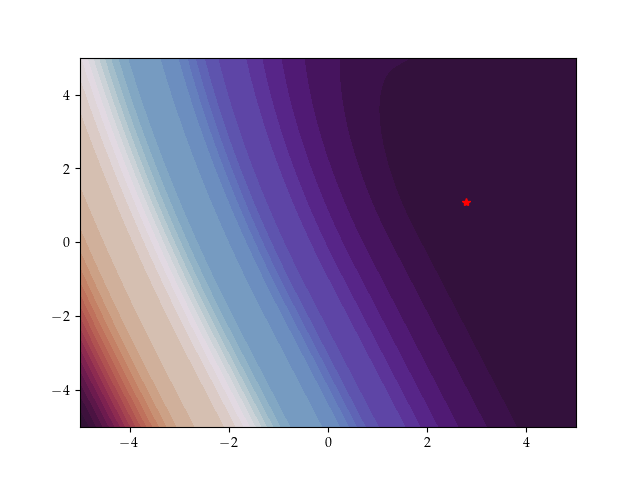
\includegraphics[trim=2.5cm 1.3cm 2.5cm 1.3cm,clip,width=\textwidth]{Figures/coco/f6.png}
    \end{minipage}
    

    \begin{minipage}[b]{0.32\textwidth}
      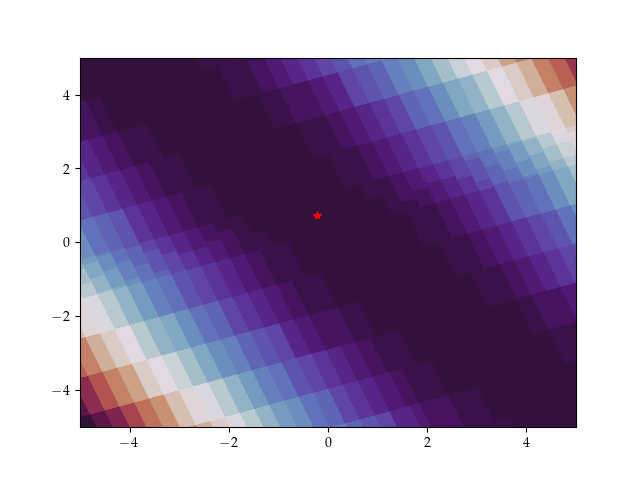
\includegraphics[trim=2.5cm 1.3cm 2.5cm 1.3cm,clip,width=\textwidth]{Figures/coco/f7.png}
    \end{minipage}
    \hfill
    \begin{minipage}[b]{0.32\textwidth}
      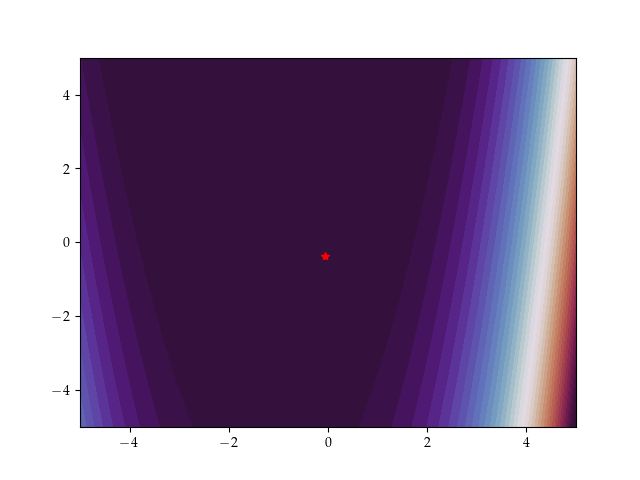
\includegraphics[trim=2.5cm 1.3cm 2.5cm 1.3cm,clip,width=\textwidth]{Figures/coco/f8.png}
    \end{minipage}
    \hfill
    \begin{minipage}[b]{0.32\textwidth}
      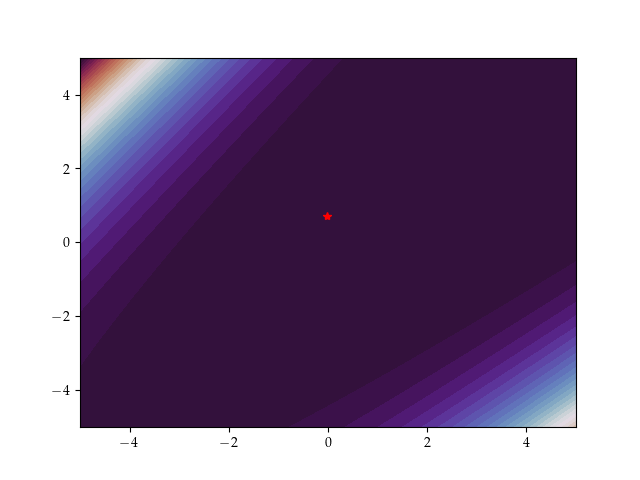
\includegraphics[trim=2.5cm 1.3cm 2.5cm 1.3cm,clip,width=\textwidth]{Figures/coco/f9.png}
    \end{minipage}
    
    \begin{minipage}[b]{0.32\textwidth}
        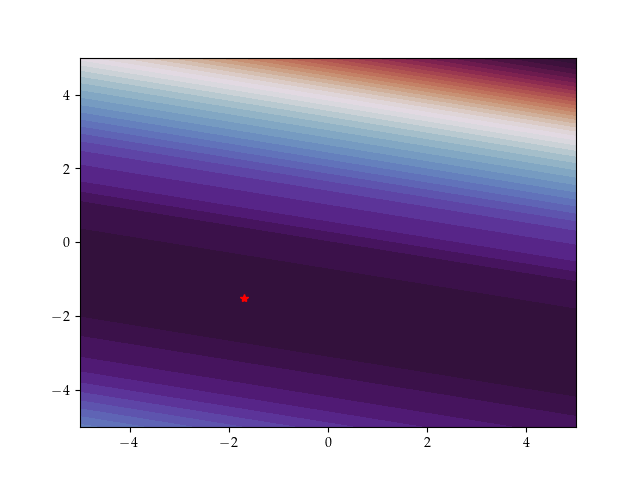
\includegraphics[trim=2.5cm 1.3cm 2.5cm 1.3cm,clip,width=\textwidth]{Figures/coco/f10.png}
    \end{minipage}
    \hfill
    \begin{minipage}[b]{0.32\textwidth}
      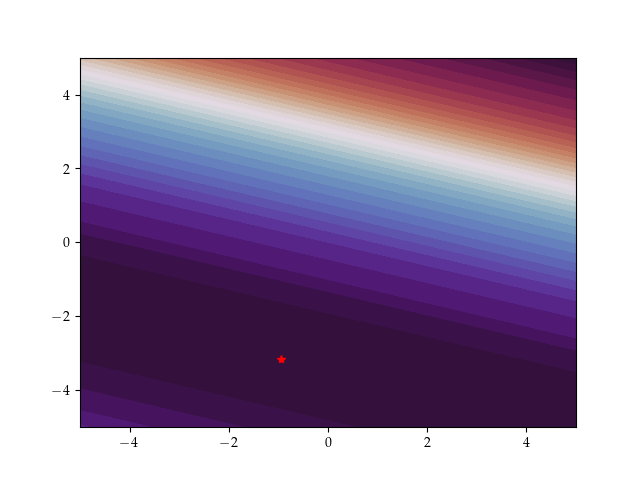
\includegraphics[trim=2.5cm 1.3cm 2.5cm 1.3cm,clip,width=\textwidth]{Figures/coco/f11.png}
    \end{minipage}
    \hfill
    \begin{minipage}[b]{0.32\textwidth}
      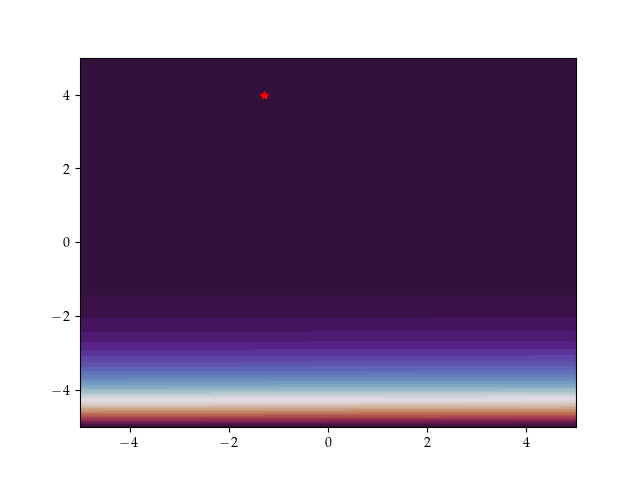
\includegraphics[trim=2.5cm 1.3cm 2.5cm 1.3cm,clip,width=\textwidth]{Figures/coco/f12.png}
    \end{minipage}
    \caption{Test functions f1 to f12}
    \label{2DBlockcyclic}
  \end{figure}
  
  \begin{figure}[h]
    \centering
    \begin{minipage}[b]{0.32\textwidth}
     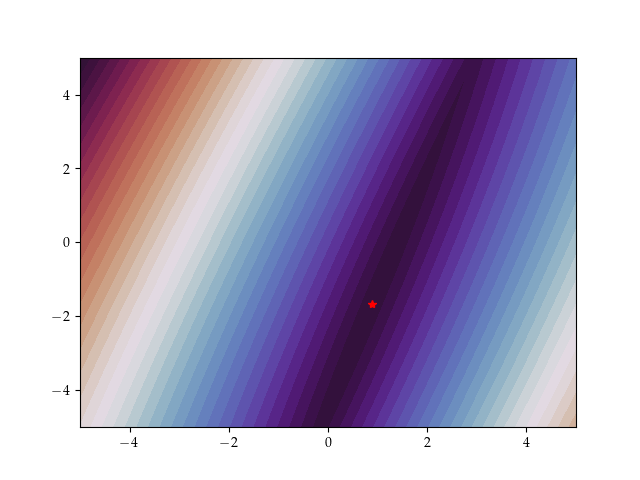
\includegraphics[trim=2.5cm 1.3cm 2.5cm 1.3cm,clip,width=\textwidth]{Figures/coco/f13.png}
    \end{minipage}
    \hfill
    \begin{minipage}[b]{0.32\textwidth}
     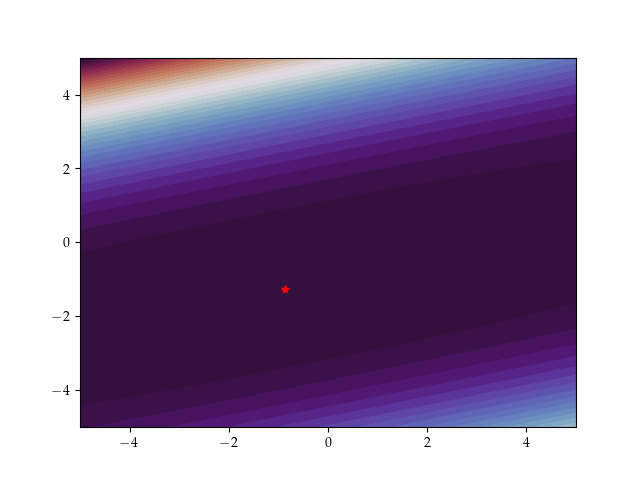
\includegraphics[trim=2.5cm 1.3cm 2.5cm 1.3cm,clip,width=\textwidth]{Figures/coco/f14.png}
    \end{minipage}
    \hfill
    \begin{minipage}[b]{0.32\textwidth}
      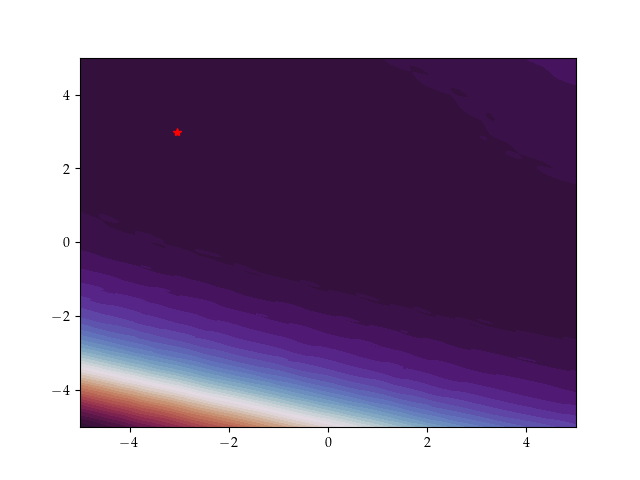
\includegraphics[trim=2.5cm 1.3cm 2.5cm 1.3cm,clip,width=\textwidth]{Figures/coco/f15.png}
      %\caption{Rank}
    \end{minipage}
    
    \begin{minipage}[b]{0.32\textwidth}
      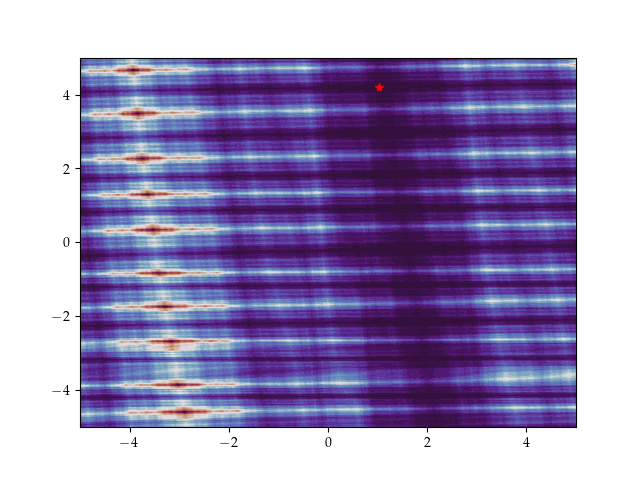
\includegraphics[trim=2.5cm 1.3cm 2.5cm 1.3cm,clip,width=\textwidth]{Figures/coco/f16.png}
    \end{minipage}
    \hfill
    \begin{minipage}[b]{0.32\textwidth}
      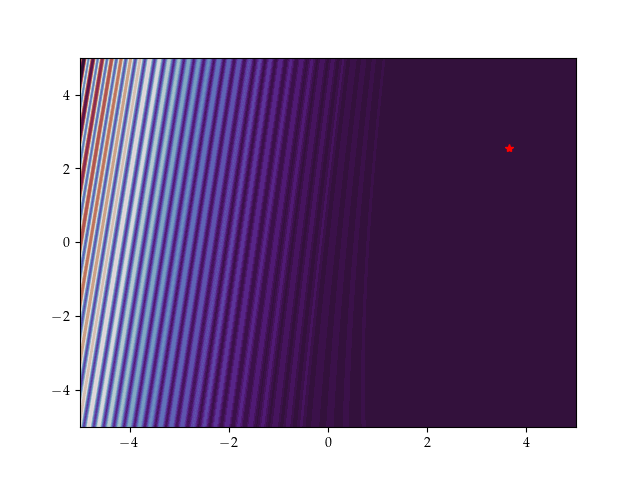
\includegraphics[trim=2.5cm 1.3cm 2.5cm 1.3cm,clip,width=\textwidth]{Figures/coco/f17.png}
    \end{minipage}
    \hfill
    \begin{minipage}[b]{0.32\textwidth}
      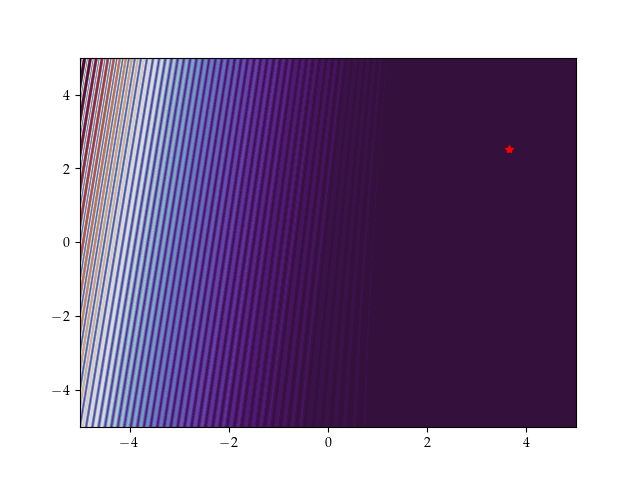
\includegraphics[trim=2.5cm 1.3cm 2.5cm 1.3cm,clip,width=\textwidth]{Figures/coco/f18.png}
    \end{minipage}
    

    \begin{minipage}[b]{0.32\textwidth}
      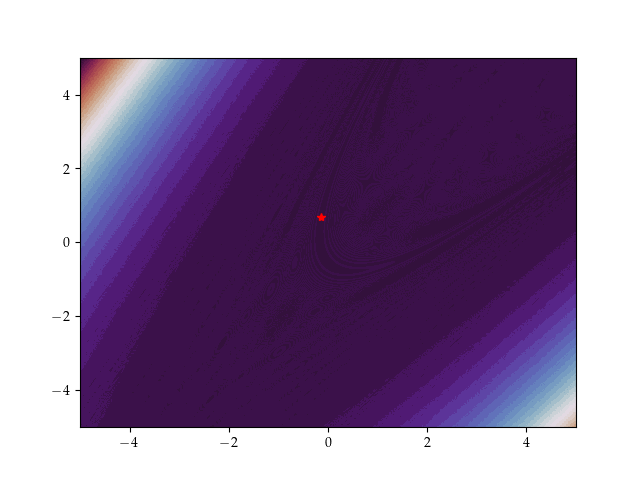
\includegraphics[trim=2.5cm 1.3cm 2.5cm 1.3cm,clip,width=\textwidth]{Figures/coco/f19.png}
    \end{minipage}
    \hfill
    \begin{minipage}[b]{0.32\textwidth}
      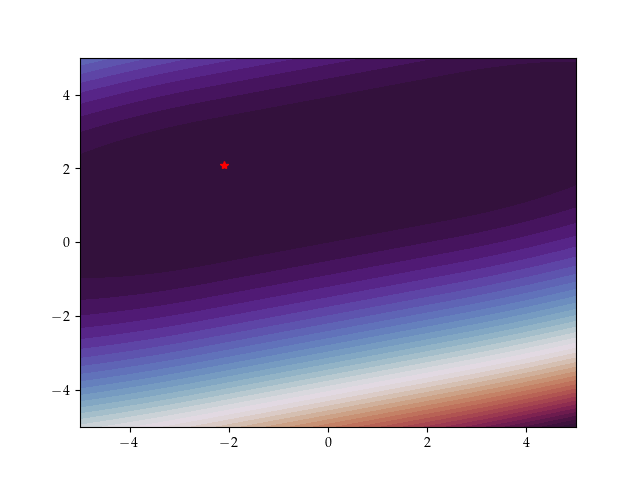
\includegraphics[trim=2.5cm 1.3cm 2.5cm 1.3cm,clip,width=\textwidth]{Figures/coco/f20.png}
    \end{minipage}
    \hfill
    \begin{minipage}[b]{0.32\textwidth}
      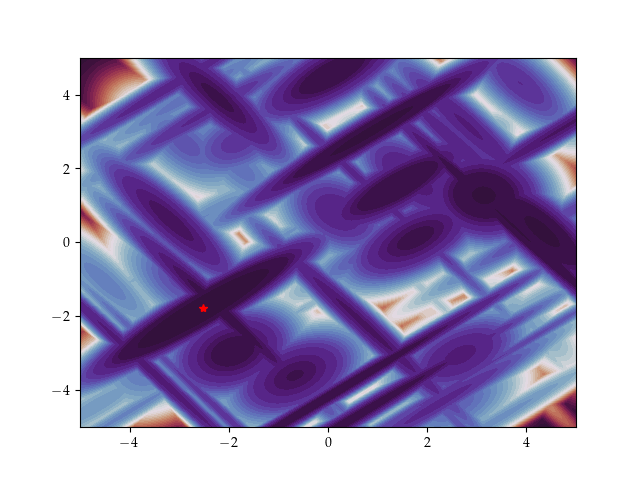
\includegraphics[trim=2.5cm 1.3cm 2.5cm 1.3cm,clip,width=\textwidth]{Figures/coco/f21.png}
    \end{minipage}
    
    \begin{minipage}[b]{0.32\textwidth}
        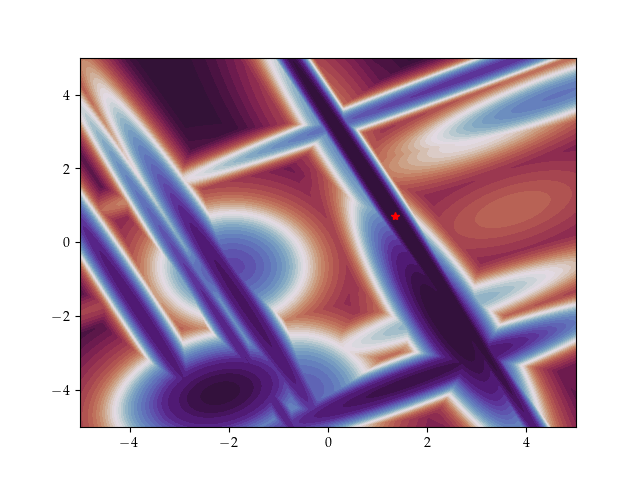
\includegraphics[trim=2.5cm 1.3cm 2.5cm 1.3cm,clip,width=\textwidth]{Figures/coco/f22.png}
    \end{minipage}
    \hfill
    \begin{minipage}[b]{0.32\textwidth}
      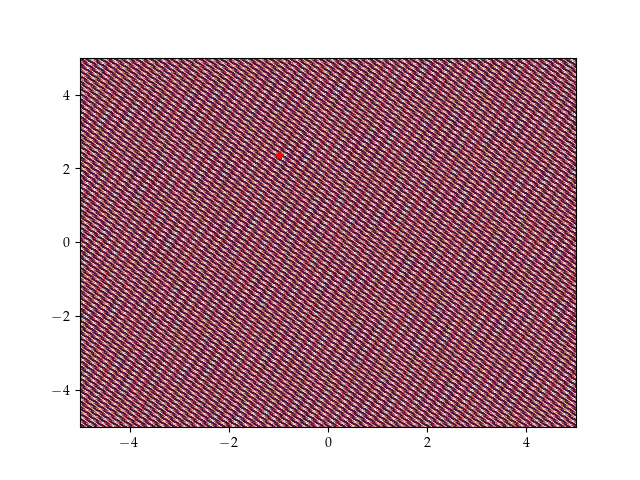
\includegraphics[trim=2.5cm 1.3cm 2.5cm 1.3cm,clip,width=\textwidth]{Figures/coco/f23.png}
    \end{minipage}
    \hfill
    \begin{minipage}[b]{0.32\textwidth}
      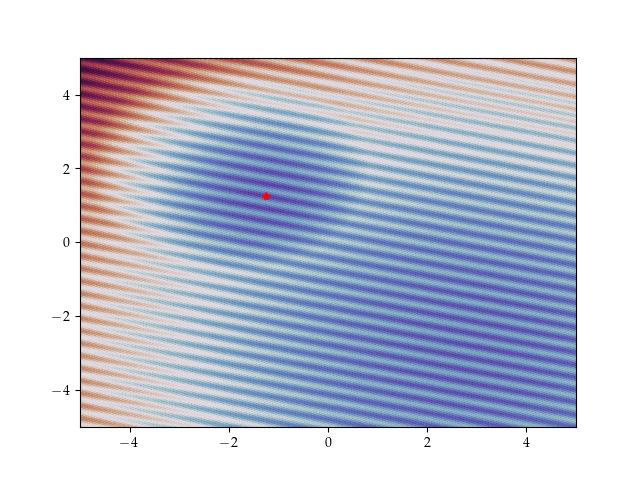
\includegraphics[trim=2.5cm 1.3cm 2.5cm 1.3cm,clip,width=\textwidth]{Figures/coco/f24.png}
    \end{minipage}
    \caption{Test functions f13-24}
    \label{f13-24}
  \end{figure}
  